\documentclass[12pt]{article}
\usepackage[margin=2.5cm]{geometry}
\usepackage{enumerate}
\usepackage{amsfonts}
\usepackage{amsmath}
\usepackage{fancyhdr}
\usepackage{amsmath}
\usepackage{amssymb}
\usepackage{amsthm}
\usepackage{mdframed}
\usepackage{graphicx}
\usepackage{subcaption}
\usepackage{adjustbox}
\usepackage{listings}
\usepackage{xcolor}
\usepackage{booktabs}
\usepackage[utf]{kotex}

\definecolor{codegreen}{rgb}{0,0.6,0}
\definecolor{codegray}{rgb}{0.5,0.5,0.5}
\definecolor{codepurple}{rgb}{0.58,0,0.82}
\definecolor{backcolour}{rgb}{0.95,0.95,0.92}

\lstdefinestyle{mystyle}{
    backgroundcolor=\color{backcolour},
    commentstyle=\color{codegreen},
    keywordstyle=\color{magenta},
    numberstyle=\tiny\color{codegray},
    stringstyle=\color{codepurple},
    basicstyle=\ttfamily\footnotesize,
    breakatwhitespace=false,
    breaklines=true,
    captionpos=b,
    keepspaces=true,
    numbers=left,
    numbersep=5pt,
    showspaces=false,
    showstringspaces=false,
    showtabs=false,
    tabsize=1
}

\lstset{style=mystyle}

\pagestyle{fancy}
\renewcommand{\headrulewidth}{0.4pt}
\lhead{Hyungmo Gu}
\rhead{CSC209 Week 9 Notes}

\begin{document}
\title{CSC209 Week 9 Notes}
\author{Hyungmo Gu}
\maketitle

\section*{Signals 1 of 2}

\bigskip

\begin{itemize}
    \item Introduction to Signals
    \begin{itemize}
        \item Signals
        \begin{itemize}
            \item are mechanisms that allow process or the os to interrupt
        currently running process and notify that an event has occured
        \end{itemize}

        \begin{center}
        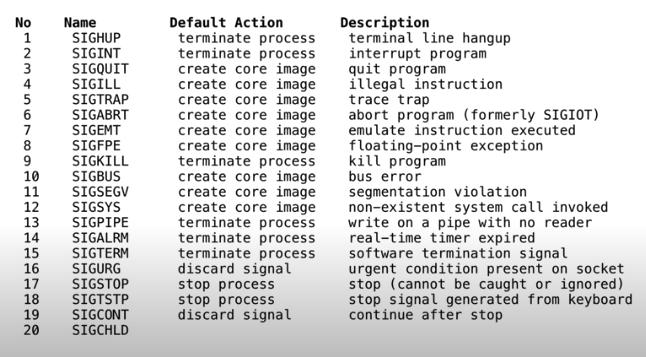
\includegraphics[width=\linewidth]{images/week_9_notes_1_1.png}
        \end{center}

        \item How it Works

        \begin{enumerate}[1.]
            \item Using hotkey
            \begin{itemize}
                \item i.e. \textit{CTRL + C} in terminal sends SIGINT
                \item i.e. \textit{CTRL + Z} in terminal sends SIGSTOP
            \end{itemize}

            \item Using kill command

            \begin{center}
            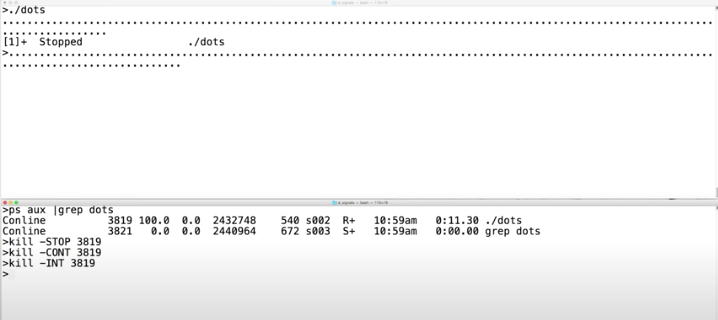
\includegraphics[width=\linewidth]{images/week_9_notes_1_2.png}
            \end{center}

    \begin{lstlisting}[language=bash]
    >>>./signals_example_1.out # <- This is done in separate terminal
    >>> ps aux | grep ./signals_example_1.out
    >>> kill -STOP <PID>
    >>> kill -CONT <PID>
    >>> kill -INT <PID>
    \end{lstlisting}

        \end{enumerate}
    \end{itemize}
\end{itemize}

\bigskip

\section*{Signals 2 of 2}

\bigskip

\begin{itemize}
    \item Signals Handling
    \begin{itemize}
        \item sigaction
        \begin{itemize}
            \item \textbf{Syntax:} int sigaction(int signum, const struct sigaction *act,
            NULL);
            \item Is a part of \textit{signal.h} library
            \item Is used to change the action taken by a process on receipt of
            a specific signal
            \item Works like try and catch in Python
            \item Don't worry about NULL :). Not knowing won't bite.
        \end{itemize}

        \bigskip

    \begin{lstlisting}[language=c]
    #include <stdio.h>
    #include <stdlib.h>
    #include <signal.h>

    void handler(int);

    int main () {
        struct sigaction newact;
        newact.sa_handler = handler; // <- like catch statement in python
        newact.sa_flags = 0;
        sigemptyset(&newact.sa_mask);
        return(0);
    }

    void handler(int code) {
        fprintf(stderr, "Signal %d caught\n", code);
    }
    \end{lstlisting}

        \begin{itemize}
            \item Use \textit{CTRL + Z} to terminate
            \item \textit{kill -KILL \textless PID \textgreater} and \textit{kill -QUIT \textless PID \textgreater}
            are two guarenteed ways to terminate a program.
        \end{itemize}

    \end{itemize}
\end{itemize}


\end{document}